
%(BEGIN_QUESTION)
% Copyright 2011, Tony R. Kuphaldt, released under the Creative Commons Attribution License (v 1.0)
% This means you may do almost anything with this work of mine, so long as you give me proper credit

Two engineers are arguing over the open-loop response of a multi-collector solar air heating process:

$$\includegraphics[width=15.5cm]{i00075x01.eps}$$

They both agree that the amount of temperature rise the air experiences from the inlet to the outlet of each collector panel is a function of the air's residence time in that collector: the slower the air moves through, the more heat it will absorb from the sun and the hotter its temperature will rise.  They also agree that this process has a lot of {\it transport delay} (dead time) from the inlet of the first panel to the outlet of the last, given the long path length the air must travel to get through all the collectors.

What they cannot agree on is how the final temperature will respond to a step-change in air flow rate (i.e. suddenly changing the blower speed).  The two engineers propose these differing open-loop responses for this system:

$$\includegraphics[width=15.5cm]{i00075x02.eps}$$

The two engineers have been arguing over this for hours because they don't have permission to actually test the system by varying the blower speed.  Their co-workers are getting really tired of hearing this argument go back and forth, and so they call you to settle it.

\vskip 10pt

Which engineer do you think is correct, and why?  Or, are neither of them correct? 

\vfil

\underbar{file i00075}
\eject
%(END_QUESTION)





%(BEGIN_ANSWER)

This is a graded question -- no answers or hints given!

%(END_ANSWER)





%(BEGIN_NOTES)

Engineer ``B'' has the better idea: air temperature will decrease in a ramp fashion to the new equilibrium point, rather than suddenly jump down as you might expect with a dead-time dominant process.

\vskip 10pt

If you imagine how each molecule of air would heat up as it traveled through the solar collectors, you would find the molecules closest to the end of the series array would experience less of a temperature drop from the increased blower speed than the molecules nearer the beginning, because the molecules near the end have already reached (nearly) full temperature.  Thus, the temperature trend will ramp downward as the nearly-full-heated molecules exit first and are followed by molecules which have had proportionately less heating. 

To illustrate in more detail, perform these thought experiments: what would happen to the temperature of an air molecule already at the outlet tube following the blower's speed increase?  Answer: no change in temperature at all, because it's already exited the collector array.  What would happen to the temperature of an air molecule exactly half-way between the second and third collectors following the blower's speed increase?  Answer: it would exit the array colder than it normally would, but not as cold as one of the air molecules just entering the array when the blower speed increases, because it's already passed through half the collector array at normal speed.  Any air molecule just entering the collector when the blower speed increases will exit the coolest of all, because it spends the least time there.

If an analogy would help, imagine a line of people being moved at a slow rate along a conveyor belt through an art museum.  The belt moves slowly so that everyone gets a chance to view the artwork.  Now imagine the conveyor belt speed suddenly increases.  Who gets the most and the least exposure to all the art following the belt's speed increase: someone at the end of the belt who already saw the museum at slow speed, someone in the middle who saw half the museum at slow speed, or someone at the beginning who saw the entire museum at high speed?  If you were to rank each person's satisfaction with their experience coming off the belt, you would begin with satisfied patrons first, then increasing dissatisfied people coming off the line, followed by the least satisfied people coming off at last.  This is what will happen to the air molecules moving through the collector array: first you'll get hot molecules exiting, followed by cooler molecules, followed by cooler-yet molecules, followed at last by the coldest molecules.  Thus, the temperature ramps down in a linear slope with the increase in blower speed.

\vskip 10pt

While this process does indeed exhibit dead time, it will not be evident as you might expect following a change in blower speed.  Where dead time will be noticed in its classic ``no response'' form is if the incoming air temperature were to suddenly change.  This change would not be seen at the outlet of the collector array until those molecules made it all the way through the array.  Until that happened, there would be no discernable change in outlet temperature (i.e. a textbook example of dead time response to a load change):

$$\includegraphics[width=15.5cm]{i00075x03.eps}$$

%INDEX% Process: solar hot-air collector process characteristics

%(END_NOTES)


